\documentclass[a4paper, titlepage]{livret} % classe spéciale rapport : livret

\usepackage[utf8]{inputenc} % accents
\usepackage[T1]{fontenc} % caractères français
\usepackage{geometry} % marges
\usepackage[francais]{babel} % langue
\usepackage{graphicx} % images
\usepackage{verbatim} % texte préformaté
\usepackage{listings} % code source
\usepackage[framed,numbered,autolinebreaks,useliterate]{mcode} % code source
\usepackage{listingsutf8} % code source accents
\usepackage[final]{pdfpages} % inclusion de pdf
\usepackage{url} % utilisation des url
\usepackage{caption} % nom des tableaux
\usepackage{amsmath} % maths
\usepackage{amsfonts, bbm} % fonts maths
\usepackage{amsthm} % théorèmes
\usepackage{pstricks} % figures
\usepackage{stmaryrd} % intervalles d'entiers
\usepackage{algorithmeUTF8} % algorithmique

\def\siecle#1{\textsc{\romannumeral #1}\textsuperscript{e}} % macro pour l'écriture des siècles
\newtheorem*{thm}{Théorème} % macro propriété
\newtheorem*{prv}{\textbf{Preuve}}
\graphicspath{{img/}} % chemin des illustrations
\DeclareSymbolFont{bbold}{U}{bbold}{m}{n}
\DeclareSymbolFontAlphabet{\mathbbold}{bbold}

\title{Projet de Probabilités} % titre
\author{Elliot Sisteron & Antoni Markovski} % auteur

\pagestyle{headings} % rappel discret (en haut à gauche)

\begin{document} % début du document

	
\includepdf{pdf/cover.pdf} % page de garde
	
	\chapter*{Introduction}
	\addcontentsline{toc}{chapter}{Introduction} % ajouter l'introduction au sommaire
		Dans notre société actuelle, où tout se réalise de plus en plus vite, la frustration de l'attente est une sensation des plus déplaisante. 
		Une manière de moins redouter cette attente est d'avoir un certain contrôle sur celle-ci. 
		En effet, de nombreuses études ont démontré que le sentiment d'impatience était très fortement lié à notre capacité à quantifier l'attente dans une situation donnée.
		
		Dans ce projet, on se propose de résoudre un problème de ce type : nous allons essayer de déterminer le temps moyen d'attente nécessaire à un passager avant l'arrivée de son bus.
		Pour cela, on sait que la durée moyenne écoulée entre le passage de deux bus est de $15$ minutes.
		On notera par la suite : 
		\begin{itemize}
			\item $(T_{n})_{n \geq 0}$ la suite de variables aléatoires réelles représentant l'horaire (exprimée en minutes) de passage de l'autobus numéro $n$. On pose $T_{0} = 0$.
			\item $(X_{n})_{n \geq 0} = (T_{n+1} - T_{n})_{n \geq 0}$ la suite de variables aléatoires qui exprime l'écart temporel entre deux passages de bus adjacents. On supposera que cette suite est constituée de variables aléatoires $i.i.d$ (indépendantes et identiquement distribuées) de loi exponentielle de paramètre $\lambda$ à déterminer.
			\item $A_{t}$ la variable aléatoire représentant l'attente nécessaire au passager pour voir un autobus passer, sachant que cet usager de la ligne est arrivé à l'instant $t > 0$ fixé. 
		\end{itemize}
		Le but sera donc ici de déterminer $\mathbb{E}[A_{t}]$.
	
		Nous commencerons par présenter le processus de Poisson pour pouvoir mieux aborder le problème.
		Dès lors, cela nous aidera à déterminer la constante $\lambda$ recherchée.
		Puis, nous nous intéresserons à la simulation de ce problème pour conjecturer le résultat attendu.
		Enfin, nous calculerons rigoureusement le temps d'attente moyen pour le comparer avec le résultat de la simulation précédente.

	\setcounter{tocdepth}{3} % profondeur table des matières
	\tableofcontents % table des matières
	
	\chapter{Présentation du processus de Poisson}
		Nous allons ici commencer par modéliser graphiquement les $v.a$ de l'énoncé pour bien comprendre le problème. 
		Nous présenterons ensuite rapidement la vie de Siméon Denis Poisson.
		Enfin, nous utiliserons une approche spécifique pour définir rigoureusement le processus de Poisson avant de déterminer $\lambda$, la constante recherchée.

		\section{Modélisation de l'expérience aléatoire}
			On est sur un espace probabilisé $(\Omega, \mathcal{F}, \mathbb{P})$.
			On s'intéresse ici aux variables aléatoires de temps (donc réelles) $(X_{n})_{n \geq 0}$ et $(T_{n})_{n \geq 0}$.
			Toutes les durées sont exprimées en minutes.\\
			$\forall n \in \mathbb{N},$ on a :
			\[\begin{array}{ccccc}
				T_{n} & : & \Omega & \to & \mathbb{R}_{+} \\
					  &   & \omega & \mapsto & T_{n}(\omega)\\
			\end{array}\]
			et,
			\[\begin{array}{ccccc}
				X_{n} & : & \Omega & \to & \mathbb{R}_{+} \\
					  &   & \omega & \mapsto & T_{n+1}(\omega) - T_{n}(\omega)\\
			\end{array}\]

			On réalise un petit schéma pour mieux visualiser les variables aléatoires mises en jeu, les $X_{n}$ représentent le temps séparant deux autobus et les $T_{n}$ évaluent l'heure de passage de chaque autobus à l'arrêt :
			\begin{figure}[!ht]
				\centering
  					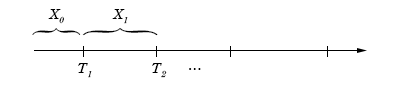
\includegraphics[scale=0.6]{g0.png}
  					\caption{Un schéma pour mieux visualiser nos v.a}
			\end{figure}

			On fixe $t > 0$. On s'intéresse à la variable aléatoire $A_{t}$ du temps d'attente d'un usager à l'arrêt.
			\[\begin{array}{ccccc}
				A_{t} & : & \Omega & \to & \mathbb{R}_{+} \\
					  &   & \omega & \mapsto & A_{t}(\omega)\\
			\end{array}\]
			Le but sera ici de déterminer la loi de $A_{t}$ pour en déduire son espérance.
			\begin{figure}[!ht]
				\centering
  					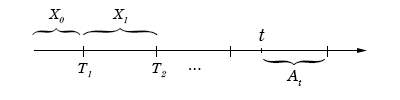
\includegraphics[scale=0.6]{g1.png}
  					\caption{Le même schéma avec $A_{t}$}
			\end{figure}

		\section{Description d'un processus de Poisson}
			\subsection{Qui est Poisson ?}
				\textsc{Siméon Denis Poisson} est un mathématicien Français du \siecle{18} – \siecle{19} siècle.
				Sa famille voulait qu'il devint médecin, et le poussa à faire des études dans ce domaine. 
				Il abandonna cette idée en 1798, pour aller étudier les mathématiques à l'École polytechnique où il fit ses études auprès de grands noms des mathématiques, notamment P. Laplace et J. Lagrange. 
				Il devint ensuite enseignant à l’Ecole polytechnique en 1802. 
				La phrase culte de ce mathématicien de renom est : \og La vie n’est bonne qu’à deux choses : découvrir des mathématiques et enseigner les mathématiques ! \fg. 

				Poisson est connu pour ses nombreuses publications en mathématiques et en sciences physiques. 
				Parmi ses publications en mathématiques pures figurent notamment une série d'articles sur les intégrales définies, et ses recherches sur les séries de Fourier ont annoncé celles de Dirichlet et de Riemann sur ce sujet.
				Il s'intéressait beaucoup aux problèmes aléatoires. 
				Le processus de Poisson est l'un des processus aléatoires les plus importants dans la théorie des probabilités. 
				Il est largement utilisé pour modéliser des points aléatoires dans le temps et l'espace, tels que les temps d'émissions radioactives, les temps d'arrivée des clients dans un centre de service, et la recherche de défauts dans des matériaux.

				Nous allons voir que plusieurs distributions de probabilités importantes apparaissent naturellement dans le processus de Poisson - la distribution de Poisson (d'où le nom donné au processus), la loi exponentielle, et la distribution gamma. 
				Le processus a une belle structure mathématique, et est utilisé comme une base pour la construction d'un certain nombre d'autres processus aléatoires, plus complexes.
				Dans notre cas, on va l'utiliser pour représenter des passages de bus à un arrêt.

			\subsection{Caractérisation du processus de Poisson par un processus de renouvellement}
				On dira qu'une suite de variables aléatoires $(T_{n})_{n \geq 0}$ est un processus de renouvellement lorsque la suite définie par $(X_{n})_{n \geq 0} = (T_{n+1} - T_{n})_{n \geq 0}$ est constituée de variable aléatoires $i.i.d$. 
				Si, de plus, les $X_{n}$ suivent une loi exponentielle de paramètre $\lambda$, on dira que les $T_{n}$ définissent un processus de Poisson d'\og intensité \fg{} $\lambda$.
				Dans notre cas, on est bien face à un processus de Poisson.

				Dans un processus de Poisson, on a donc que : $\forall n \geq 0, \ X_{n} \hookrightarrow \xi(\lambda)$.
				La densité de probabilité de $X_{n}$ est ainsi définie :
				\[
					\forall x \in \mathbb{R}, \ f_{X_{n}}(x) = \lambda e^{-\lambda x} \mathbbm{1}_{\mathbb{R}_{+}}(x)
				\]
				On peut donc en déduire la fonction de répartition $F_{X_{n}}$ de chacune de ces variables aléatoires
				\[\begin{aligned}
					\forall x \in \mathbb{R}, \ F_{X_{n}}(x) & = \mathbb{P}(X_{n} \leq x) \\
							     						     & = \int_{-\infty}^{x} f_{X_{n}}(t)dt\\
								 						     & = \int_{-\infty}^{x} \lambda e^{-\lambda t} \mathbbm{1}_{\mathbb{R}_{+}}(t)dt \\
								 						     & = \int_{0}^{x} \lambda e^{-\lambda t}dt \\
								 						     & = \lambda \left[-\frac{1}{\lambda} e^{-\lambda t}\right]_{0}^{x}\\
								 						     & = \left(1 - e^{-\lambda x}\right)\mathbbm{1}_{\mathbb{R}_{+}}(x)\\
				\end{aligned}\]

			\subsection{Processus de comptage}
				Une autre manière de définir le processus de Poisson serait à partir de $N_{t}$ (pour $t > 0$ fixé), la variable aléatoire qui \og compte \fg{} le nombre de $T_{n}$ déjà produits à l'instant $t$.
				Autrement dit, 
				\[
					N_{t} = \sum_{n \geq 0} \mathbbm{1}_{\{T_{n} \leq t\}}
				\]
				\[\begin{array}{ccccc}
					N_{t} & : & \Omega & \to & \mathbb{N} \\
					  	  &   & \omega & \mapsto & \sum_{n \geq 0} \mathbbm{1}_{\{T_{n} \leq t\}}(\omega)\\
				\end{array}\]
				On a donc la relation suivante :
				\[\begin{aligned}
					\forall \omega \in \Omega, \ \forall n \in \mathbb{N}, \ N_{t}(\omega) = n & \Leftrightarrow \forall k \in \llbracket 1;n \rrbracket, \ \mathbbm{1}_{\{T_{k} \leq t\}}(\omega) = 1 \ et \ \forall k > n, \ \mathbbm{1}_{\{T_{k} \leq t\}}(\omega) = 0\\
																							   & \Leftrightarrow \forall k \in \llbracket 1;n \rrbracket, \ T_{k}(\omega) \leq t \ et \ \forall k > n, \ T_{k}(\omega) > t\\
														  									   & \Leftrightarrow T_{n}(\omega) \leq t < T_{n + 1}(\omega)
				\end{aligned}\]

				Ici, la variable aléatoire $N_{t}$ compte le nombre de bus passés dans l'intervalle de temps $[0;t]$.
				On aurait aussi pu s'intéresser à la variable aléatoire de comptage dans un intervalle quelconque $N_{]a;b]}$\footnote{Étudiée dans l'annexe A}.
				\begin{figure}[!ht]
					\centering
  						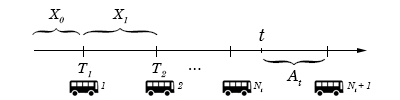
\includegraphics[scale=0.6]{g2.png}
  						\caption{Un schéma pour visualiser $N_{t}$}
				\end{figure}

				On ne va pas caractériser le processus de Poisson avec $N_{t}$, mais nous allons tout de même étudier sa loi à partir de la loi des $T_{n}$.
				En effet :
				\[\begin{aligned}
					\omega \in \{N_{t} = n\} & \Leftrightarrow \omega \in \{T_{n} \leq t < T_{n + 1}\} \\
											 & \Leftrightarrow \omega \in \{T_{n} \leq t\} \cap \{t < T_{n + 1}\}
				\end{aligned}\]
				Donc, 
				\[\begin{aligned}
					\mathbb{P}(N_{t} = n) & = \mathbb{P}(T_{n} \leq t \cap t < T_{n + 1}) \\
										  & = \mathbb{P}(T_{n} \leq t) +  \mathbb{P}(T_{n + 1} > t) - \mathbb{P}(T_{n} \leq t \cup t < T_{n + 1})\\
										  & = F_{T_{n}}(t) +  1 - F_{T_{n+1}}(t) - 1\\
				\end{aligned}\]
				Car
				\[\begin{aligned}
					\omega \in \{T_{n} \leq t \cup t < T_{n + 1}\} & \Leftrightarrow \omega \in \{T_{n} \leq t\} \ ou \ \omega \in \{t < T_{n + 1}\}\\
																   & \Leftrightarrow \omega \in \Omega\\
				\end{aligned}\]
				D'où :
				\[\boxed{
					\forall n \in \mathbb{N}, \ \mathbb{P}(N_{t} = n) = F_{T_{n}}(t) - F_{T_{n+1}}(t)
				}\]
				Il nous reste à trouver la loi de des $T_{n}$.
				On remarque pour cela que, par somme télescopique :
				\[
					\forall n \in \mathbb{N}^{*}, \ T_{n} = \sum_{k = 0}^{n-1} X_{k}
				\]
				Or, on rappelle que pour deux variables aléatoires réelles $X$ et $Y$ indépendantes admettant des densités de probabilités $f_{X}$ et $f_{Y}$, la densité de leur somme $f_{X+Y}$ est donnée par le produit de convolution :
				\[
					\forall x \in \mathbb{R}, \ f_{X+Y}(x) = (f_{X}*f_{Y})(x) = \int_{-\infty}^{\infty} f_{X}(t)f_{Y}(x-t)dt
				\]
				On peut donc retrouver la densité de probabilité de $T_{n}$ par récurrence.
				$T_{1} = X_{0} \hookrightarrow \xi(\lambda)$, donc :
				\[
					f_{T_{1}}(x) = f_{X_{0}}(x) = \lambda e^{-\lambda x}\mathbbm{1}_{\mathbb{R}_{+}}(x)
				\]
				$T_{2} = X_{0} + X_{1}$, ainsi :
				\[\begin{aligned}
					f_{T_{2}}(x) = f_{X_{0} + X_{1}}(x) & = \int_{-\infty}^{\infty} f_{X_{0}}(t)f_{X_{1}}(x-t)dt\\
														& = \int_{-\infty}^{\infty} \lambda e^{-\lambda t}\mathbbm{1}_{\mathbb{R}_{+}}(t)\lambda e^{-\lambda (x-t)}\mathbbm{1}_{\mathbb{R}_{+}}(x-t)dt\\
														& = \lambda^{2} e^{-\lambda x}\int_{0}^{x}dt\\
														& = \lambda^{2} x e^{-\lambda x} \mathbbm{1}_{\mathbb{R}_{+}}(x)\\
				\end{aligned}\]
				$T_{3} = T_{2} + X_{2}$, d'où :
				\[\begin{aligned}
					f_{T_{3}}(x) = f_{T_{2} + X_{2}}(x) & = \int_{-\infty}^{\infty} f_{T_{2}}(t)f_{X_{2}}(x-t)dt\\
														& = \int_{-\infty}^{\infty} \lambda^{2} t e^{-\lambda t}\mathbbm{1}_{\mathbb{R}_{+}}(t)\lambda e^{-\lambda (x-t)}\mathbbm{1}_{\mathbb{R}_{+}}(x-t)dt\\
														& = \lambda^{3} e^{-\lambda x}\int_{0}^{x} t dt\\
														& = \lambda^{3} \frac{x^{2}}{2} e^{-\lambda x} \mathbbm{1}_{\mathbb{R}_{+}}(x)\\
				\end{aligned}\]
				On peut ainsi conjecturer que :
				\[\boxed{
					\forall n \in \mathbb{N}^{*}, \ \forall x \in \mathbb{R}, \ f_{T_{n}}(x) = \lambda^{n} \frac{x^{n-1}}{(n-1)!} e^{-\lambda x} \mathbbm{1}_{\mathbb{R}_{+}}(x)
				}\]

				L'initialisation est déjà faite, il suffit de montrer l'hérédité. Supposons la propriété correcte au rang $n \in \mathbb{N}^{*}$ fixé.\\
				$T_{n+1} = T_{n} + X_{n}$, donc :
				\[\begin{aligned}
					f_{T_{n+1}}(x) = f_{T_{n} + X_{n}}(x) & = \int_{-\infty}^{\infty} f_{T_{n}}(t)f_{X_{n}}(x-t)dt\\
														  & = \int_{-\infty}^{\infty} \lambda^{n} \frac{t^{n-1}}{(n-1)!} e^{-\lambda t}\mathbbm{1}_{\mathbb{R}_{+}}(t)\lambda e^{-\lambda (x-t)}\mathbbm{1}_{\mathbb{R}_{+}}(x-t)dt\\
														  & = \frac{\lambda^{n+1}}{(n-1)!} e^{-\lambda x}\int_{0}^{x} t^{n-1} dt\\
														  & = \lambda^{n+1} \frac{x^{n}}{n!} e^{-\lambda x} \mathbbm{1}_{\mathbb{R}_{+}}(x)\\
				\end{aligned}\]
				Ainsi, on peut en déduire que la conjecture précédente est vraie.
				On remarque au passage que $T_{n} \hookrightarrow \Gamma(n,\lambda)$.
				On aurait pu s'attendre à ce résultat, vu que la somme de $n$ variables exponentielles $i.i.d$ de paramètre $\lambda$ suit une loi gamma de paramètre $n$ et $\lambda$.

				Pour en déduire la loi de $T_{n}$, il nous reste maintenant à étudier la fonction de répartition de $T_{n}$ : 
				\[\begin{aligned}
					\forall n \in \mathbb{N}^{*}, \ \forall x \in \mathbb{R}, \ F_{T_{n}}(x) & = \mathbb{P}(T_{n} \leq x) \\ 
																							 & = \int_{-\infty}^{x} \lambda^{n} \frac{t^{n-1}}{(n-1)!} e^{-\lambda t} \mathbbm{1}_{\mathbb{R}_{+}}(t)dt\\ 
																							 & = \frac{\lambda^{n}}{(n-1)!} \int_{0}^{x} t^{n-1} e^{-\lambda t}dt
				\end{aligned}\]
				On pose :
				\[
					I_{n}(x) = \int_{0}^{x} t^{n-1} e^{-\lambda t}dt
				\]
				On va encore utiliser une récurrence\footnote{Voir l'annexe B pour une autre démonstration plus élégante} sur $n$ pour calculer $I_{n}$.
				Commençons par conjecturer le résultat en utilisant une intégration par partie, on fixe $x \in \mathbb{R}_{+}$ et $n \in \mathbb{N}^{*}$ :
				\[\begin{aligned}
					I_{n}(x) & = \int_{0}^{x} t^{n-1} e^{-\lambda t}dt \\
						  	 & = \left[ -\frac{t^{n-1}}{\lambda} e^{-\lambda t}\right]_{0}^{x} - \int_{0}^{x} - (n-1)\frac{t^{n-2}}{\lambda} e^{-\lambda t}dt\\
						     & = -\frac{x^{n-1}}{\lambda} e^{-\lambda x} - (n-1)\frac{x^{n-2}}{\lambda^{2}} e^{-\lambda x} - ... -\frac{(n-1)!}{1!}\frac{x}{\lambda^{n-1}} e^{-\lambda x} - \frac{(n-1)!}{\lambda^{n}} e^{-\lambda x} + \frac{(n-1)!}{\lambda^{n}}\\
				\end{aligned}\]
				On se doute donc que $I_{n}$ sera de la forme :
				\[\begin{aligned}
					I_{n}(x) & = \frac{(n-1)!}{\lambda^{n}} -e^{-\lambda x} \sum_{k = 1}^{n} \frac{(n-1)!}{(n-k)!}\frac{x^{n-k}}{\lambda^{k}}\\
						  	 & = \frac{(n-1)!}{\lambda^{n}} -e^{-\lambda x} \sum_{k = 0}^{n-1} \frac{(n-1)!}{k!}\frac{(\lambda x)^{k}}{\lambda^{n}}\\
				\end{aligned}\]
				En effet, pour ce qui est de l'initialisation, à $x \in \mathbb{R}_{+}$ fixé :
				\[\begin{aligned}
					I_{1}(x) &_= \int_{0}^{x} e^{-\lambda t}dt \\
						  	 &_= \frac{1}{\lambda}(1 - e^{-\lambda x})\\
						  	 & = \frac{(1-1)!}{\lambda^{1}} -e^{-\lambda x} \frac{(1-1)!}{0!}\frac{(\lambda x)^{0}}{\lambda^{1}}\\
				\end{aligned}\]
				Ce qui vérifie la propriété au rang $1$.
				On s'occupe de l'hérédité, supposons la propriété au rang $n$, calculons $I_{n+1}$ (toujours à $x \in \mathbb{R}_{+}$ fixé) :
				\[\begin{aligned}
					I_{n+1}(x) &_= \int_{0}^{x} t^{n} e^{-\lambda t}dt \\
						  	   &_= -\frac{1}{\lambda}\left[t^{n} e^{-\lambda t}\right]_{0}^{x} + \frac{n}{\lambda} I_{n}\\
						  	   & = -\frac{x^{n}}{\lambda}e^{-\lambda x} + \frac{n}{\lambda}\frac{(n-1)!}{\lambda^{n}} - \frac{n}{\lambda}e^{-\lambda x} \sum_{k = 0}^{n-1} \frac{(n-1)!}{k!}\frac{(\lambda x)^{k}}{\lambda^{n}}\\
						  	   & = \frac{n!}{\lambda^{n+1}} - e^{-\lambda x} \sum_{k = 0}^{n} \frac{n!}{k!}\frac{(\lambda x)^{k}}{\lambda^{n+1}}\\
				\end{aligned}\]
				Finalement, on a bien :
				\[\boxed{
					\forall n \in \mathbb{N}^{*}, \ \forall x \in \mathbb{R}, \ I_{n}(x)_= \left(\frac{(n-1)!}{\lambda^{n}} -e^{-\lambda x} \sum_{k = 0}^{n-1} \frac{(n-1)!}{k!}\frac{(\lambda x)^{k}}{\lambda^{n}}\right)\mathbbm{1}_{\mathbb{R}_{+}}(x)
				}\]
				D'où :
				\[\begin{aligned}
					\forall n \in \mathbb{N}^{*}, F_{T_{n}}(x) & = \frac{\lambda^{n}}{(n-1)!} I_{n}(x)\\
															   & = \left(1 -e^{-\lambda x} \sum_{k = 0}^{n-1} \frac{1}{k!}\frac{(\lambda x)^{k}}{1}\right)\mathbbm{1}_{\mathbb{R}_{+}}(x)\\
				\end{aligned}\]
				N'oublions pas le cas où $n = 0$,
				\[
					F_{T_{0}}(x) = \mathbb{P}(T_{0} \leq x) = \mathbb{P}(0 \leq x) = \mathbbm{1}_{\mathbb{R}_{+}}(x)
				\]
				Donc la loi de $T_{n}$ est bien définie par :
				\[\boxed{
					\forall n \in \mathbb{N}, \ \forall x \in \mathbb{R}, \ F_{T_{n}}(x) = \left(1 -e^{-\lambda x} \sum_{k = 0}^{n-1} \frac{(\lambda x)^{k}}{k!}\right)\mathbbm{1}_{\mathbb{R}_{+}}(x)\\
				}\]
				Et finalement, il en découle la loi de $N_{t}$ :
				\[\begin{aligned}
					\mathbb{P}(N_{t} = n) & = F_{T_{n}}(t) - F_{T_{n+1}}(t)\\
										  & = 1 -e^{-\lambda t} \sum_{k = 0}^{n-1} \frac{(\lambda t)^{k}}{k!} - 1 + e^{-\lambda t} \sum_{k = 0}^{n} \frac{(\lambda t)^{k}}{k!}\\
										  & = e^{-\lambda t}\frac{(\lambda t)^{n}}{n!}
				\end{aligned}\]
				Ainsi,
				\[\boxed{
					\forall n \in \mathbb{N}, \ \mathbb{P}(N_{t} = n) = e^{-\lambda t}\frac{(\lambda t)^{n}}{n!}
				}\]
				On remarque que $N_{t}$ suit une loi de Poisson de paramètre $\lambda t$, on comprend alors mieux l'appellation \og processus de Poisson \fg{} : $N_{t} \hookrightarrow \mathcal{P}(\lambda t)$.

		\section{Détermination de $\lambda$}
			On sait que la durée moyenne entre deux passages de bus est de $15$ minutes.
			Ainsi, on peut en déduire que :
			\[
				\forall n \geq 0, \ \mathbb{E}[X_{n}] = 15
			\]

			Or, on sait que chaque $X_{n} \hookrightarrow \xi(\lambda)$.
			Nous avons donc besoin de calculer l'espérance d'une variable aléatoire de loi exponentielle.

			\subsection{Calcul de l'espérance d'une variable aléatoire suivant une loi exponentielle}
				Soit $X$ une variable aléatoire réelle sur un espace probabilisé $(\Omega, \mathcal{F}, \mathbb{P})$ telle que $X \hookrightarrow \xi(\lambda)$.
				Soit $f_{X}$ sa densité de probabilité.
				
				Par le théorème de transfert, on a que :
				$\begin{aligned}[t]
   					\mathbb{E}[X] & = \int_{-\infty}^{\infty} t f_{X}(t)dt \\
                                  & = \int_{-\infty}^{\infty} t \lambda e^{-\lambda t} \mathbbm{1}_{\mathbb{R}_{+}} (t) dt \\
                                  & = \lambda \int_{0}^{\infty} t e^{-\lambda t} dt \\
 				\end{aligned}$

 				Par une intégration par partie, il en résulte que :
 				$\begin{aligned}[t]
   					\mathbb{E}[X] & = \lambda \left(\left[ -\frac{t}{\lambda} e^{-\lambda t}\right]_{0}^{\infty} - 
   										\int_{0}^{\infty} -\frac{1}{\lambda} e^{-\lambda t} dt\right) \\
                                  & = \lambda \left[-\frac{1}{\lambda^{2}} e^{-\lambda t}\right]_{0}^{\infty} \\
                                  & = \frac{1}{\lambda} \\
 				\end{aligned}$

 				D'où :
 				\[\boxed{
 					\mathbb{E}[X] = \frac{1}{\lambda}
 				}\]
 			\subsection{Calcul de $\lambda$}
				On peut ainsi en déduire $\lambda$ :
				\[\begin{aligned}[t]
					\forall n \geq 0, \ \mathbb{E}[X_{n}] = 15 & \Leftrightarrow \frac{1}{\lambda} = 15 \\
										   				& \Leftrightarrow \lambda = \frac{1}{15} \\
				\end{aligned}\]
				D'où :
 				\[\boxed{
 					\lambda = \frac{1}{15}
 				}\]

	\chapter{Simulation et estimation de $\mathbb{E}[A_{t}]$}
		Ici, on s'intéressera d'abord à la simulation de variables aléatoires réelles, puis à la simulation de $v.a$ exponentielles pour pouvoir enfin simuler $A_{t}$.
		On émettra d'abord une conjecture préliminaire concernant son espérance, puis nous la simulerons pour en déduire une conjecture plus affinée.

		\section{Comment simuler une variable aléatoire réelle ?}
			Soit $X$ une variable aléatoire réelle sur un espace probabilisé $(\Omega, \mathcal{F}, \mathbb{P})$.
			On connaît la loi de $X$, c'est-à-dire la fonction de répartition $F_{X}$ telle que $\forall x \in \mathbb{R}, \ F_{X}(x) = \mathbb{P}(X \leq x)$.
			On cherche ici à simuler la $v.a.r \ X$ sur $(\Omega, \mathcal{F}, \mathbb{P})$.
			Pour cela, on supposera que l'on est déjà capable de simuler la loi uniforme $\mathcal{U}([0;1])$ (par exemple, la fonction $rand()$ en C est capable de simuler une telle loi).

			On pose $G_{X}$ l'application telle que $\forall u \in [0;1[, \ G_{X}(u) = \inf{\{t \in \mathbb{R} \ / \ F_{X}(t) > u\}}$ aussi appelée \og inverse généralisée de $F_{X}$ \fg.
			En effet, pour $F_{X}$ continue et strictement croissante, on a $G_{X} = F_{X}^{-1}$.
			On remarque que cette fonction est croissante et \textit{càdlàg} (c'est-à-dire continue à droite et limitée à gauche) du fait que $F_{X}$ est croissante et \textit{càdlàg}.

			\begin{thm}
				Si $U \hookrightarrow \mathcal{U}([0;1])$, $G_{X}(U)$ a la même loi que $X$.
			\end{thm}
			\begin{prv}
				Calculons la $f.d.r$ $F_{G_{X}(U)}$ de $G_{X}(U)$.
				Soit $x \in \mathbb{R}$ :
				\[
					F_{G_{X}(U)}(x) = \mathbb{P}(G_{X}(U) \leq x)
				\]
				Or, $\forall u \in [0;1[$
				\[\begin{aligned}[t]
					x < G_{X}(u) & \Rightarrow x < \inf{\{t \in \mathbb{R} \ / \ F_{X}(t) > u\}}\\
								 & \Rightarrow F_{X}(x) \leq u \\
				\end{aligned}\]
				Donc, par contraposée,
				\[\boxed{
					F_{X}(x) > u \Rightarrow x \geq G_{X}(u)
				}\]
				Et, du fait de la croissance de $F_{X}$,
				\[
					x \geq G_{X}(u) \Rightarrow F_{X}(x) \geq F_{X}(G_{X}(u))
				\]
				Or, comme $F_{X}$ est \textit{càdlàg}, il existe $(t_{n})_{n}$ une suite de réels décroissante telle que $\forall n \in \mathbb{N}, \ F_{X}(t_{n}) > u$ et $t_{n} \underset{n \to +\infty}{\longrightarrow} G_{X}(u)$.
				Ainsi, $F_{X}(G_{X}(u)) \geq u$.
				D'où :
				\[\boxed{
					x \geq G_{X}(u) \Rightarrow F_{X}(x) \geq u
				}\]
				En revenant au calcul de la fonction de répartition précédente, on peut ainsi en déduire :
				\[\begin{aligned}[t]
					F_{G_{X}(U)}(x) & = \mathbb{P}(G_{X}(U) \leq x)\\
									& = \mathbb{P}(U < F_{X}(x))
				\end{aligned}\]
				Or, la $f.d.r$ de $U$ est continue, donc $\mathbb{P}(U = F_{X}(x)) = 0$, donc $\mathbb{P}(U < F_{X}(x)) = \mathbb{P}(U \leq F_{X}(x))$.
				D'où :
				\[\begin{aligned}[t]
					F_{G_{X}(U)}(x) & = \mathbb{P}(U \leq F_{X}(x))\\
									& = F_{U}(F_{X}(x)) \\
									& = F_{X}(x) \\
				\end{aligned}\]
				car $F_{X}(x)$ est à valeurs dans $[0;1]$.

				Ainsi par le théorème de caractérisation d'une loi par sa $f.d.r$, on obtient que la loi de $X$ est la même que la loi de $G_{X}(U)$.
			\end{prv}

			D'après ce théorème, on peut donc simuler n'importe quelle variable aléatoire réelle en trouvant son inverse généralisée.

			\subsection{Simulation d'une variable aléatoire exponentielle}
				On a vu que pour simuler une $v.a$ exponentielle il fallait trouver son inverse généralisée.
				Or, ici, on remarque que la $f.d.r$ de notre loi exponentielle est bijective donc $G_{X} = F_{X}^{-1}$.
				Trouvons cette fonction réciproque :
				\[\begin{aligned}[t]
					\forall x \in \mathbb{R}_{+}, \ F_{X}(x) = u & \Leftrightarrow 1 - e^{-\lambda x} = u \\
									& \Leftrightarrow e^{-\lambda x} = 1 - u\\
									& \Leftrightarrow x = -\frac{ln(1 - u)}{\lambda} \\
				\end{aligned}\]
				Donc, 
				\[
					F_{X}^{-1}(u) = -\frac{ln(1 - u)}{\lambda}
				\]

				Finalement, pour simuler la loi d'un $v.a$ exponentielle, il suffit d'appliquer $F_{X}^{-1}(u)$ sur une distribution de $u \in [0; 1[$ uniforme.
				On peut même prendre :
				\[\boxed{
					\forall u \in ]0;1], \ F_{X}^{-1}(u) = -\frac{ln(u)}{\lambda}
				}\]
				ce qui revient exactement au même et facilite les calculs.

		\section{Conjecture préliminaire}
			D'après les données, il semble intuitif de conjecturer que le temps d'attente moyen d'un usager à l'arrêt de bus sera de $7.5$ minutes.
			En effet, on sait qu'en moyenne les intervalles $X_{n}$ ont pour longueur 15 minutes.
			La logique voudrait, sachant qu'un utilisateur arrivera à un horaire $t$ tiré au sort de manière uniforme, que la moyenne du temps d'attente soit moitié moindre.
			Si l'on ne se représente que des intervalles $X_{n}$ de durée moyenne, alors la moyenne du temps d'attente dans un tel intervalle sera clairement de la moitié de cette durée.
			\begin{figure}[!ht]
				\centering
  					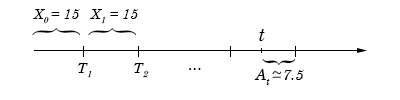
\includegraphics[scale=0.6]{g4.png}
  					\caption{Notre première conjecture}
			\end{figure}
			\newpage

		\section{Simulation de $A_{t}$}
			\subsection{Algorithme de simulation}
				On rappelle que $A_{t}$ est la variable aléatoire représentant le temps à attendre avant l'arrivée d'un bus.
				Simuler $A_{t}$, après avoir simulé un horaire $t > 0$ de manière uniforme, c'est donc :
				\begin{enumerate}
					\item Simuler le processus de Poisson en générant et sommant les $X_{n}$ qui suivent une loi exponentielle de paramètre $\lambda$.
					\item S'arrêter quand l'intervalle dans lequel se trouve $t$ est atteint : il s'agit de $[T_{N_{t}}; T_{N_{t}+1}[$.
					\item En déduire $A_{t} = T_{N_{t}+1} - t$.
				\end{enumerate}

				Nous allons formaliser cet algorithme en pseudo-language.
				On suppose que l'on connaît une fonction $simulerUneLoiUniforme(a,b)$ qui nous permet de simuler $U \hookrightarrow \mathcal{U}_{[a;b]}$.
				Lors de l'implémentation en langage C de cet algorithme, nous utiliserons la fonction $rand()$ pour en déduire $U = a + (b-a)rand()/((double)RAND\_MAX))$.

				\begin{figure}[!ht]
					\begin{algorithme}
						\fonction{simulerUneLoiExponentielle}{lambda : \reel}{\reel}
							{}
							{
								\retourner{-$ln$(simulerUneLoiUniforme(0,1))/lambda}
							}
					\end{algorithme}
					\caption{L'algorithme de simulation d'une loi exponentielle}
				\end{figure}

				\begin{figure}[!ht]
					\begin{algorithme}
						\fonction{simulerAt}{t : \reel, lambda : \reel}{\reel}
							{somme : \reel}
							{
								\affecter{somme}{0}
								\tantque{(somme $<$ t)}
								{
									\affecter{somme}{somme + simulerUneLoiExponentielle(lambda)}
								}
								\retourner{(somme - t)}
							}
					\end{algorithme}
					\caption{L'algorithme de simulation de $A_{t}$}
				\end{figure}

				Il ne nous restera qu'à faire la moyenne d'un certain nombre de simulations de $A_{t}$ pour avoir un ordre d'idée de $\mathbb{E}(A_{t})$, pour ainsi savoir si notre conjecture est correcte.

				\begin{figure}[!ht]
					\begin{algorithme}
						\fonction{simulerEsperanceAt}{t : \reel, lambda : \reel, nbEssais : \naturelNonNul}{\reel}
							{somme : \reel, i : \naturelNonNul}
							{
								\affecter{somme}{0}
								\pour{i}{1}{nbEssais}{}
								{
									\affecter{somme}{somme + simulerAt(t, lambda)}
								}
								\retourner{somme/nbEssais}
							}
					\end{algorithme}
					\caption{L'algorithme de calcul de l'espérance de $A_{t}$}
				\end{figure}

			\subsection{Implémentation de l'algorithme en langage C}
				On se propose de réaliser un petit programme en C pour estimer l'espérance de $A_{t}$.
				En plus d'être un langage portable, important pour comprendre le fonctionnement d'un ordinateur (on entend par là proche de la machine, ou \og langage de bas niveau \fg{}), le C est aussi modulaire.
				C'est pourquoi nous avons ici séparé notre code source en différents modules, ce qui nous permet deux choses :
				\begin{enumerate}
					\item Une meilleure répartition du travail, le programme étant scindé en \og boîtes noires \fg{} pour que chaque membre du binôme puisse concevoir sa partie sans se soucier du travail de l'autre
					\item Une séparation plus claire et plus efficace pour une meilleure réutilisabilité (ce ne sera pas notre dernier projet en C, autant prévoir pour les prochains).
				\end{enumerate}

				Ainsi, on peut distinguer différents fichiers où sont regroupées fonctions et procédures spécifiques à certaines tâches :

				\begin{figure}[!ht]
					\centering
  						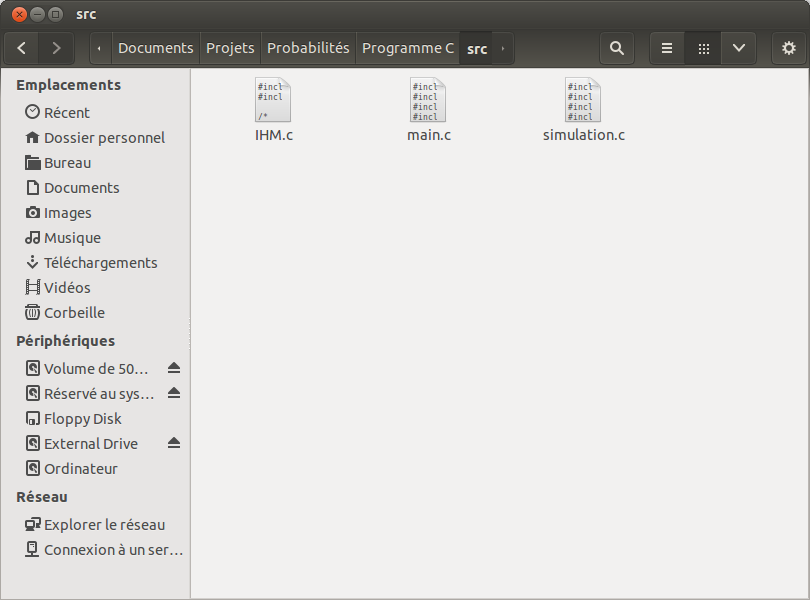
\includegraphics[scale = 0.38]{captureFichiers.png}
  						\caption{Les fichiers source utilisés par notre programme}
				\end{figure}

				\begin{itemize}
					\item Le \textit{main}
					\item Le module \textit{IHM} (Interface Homme Machine) où sont regroupées des fonctions de saisie et d'affichage sur l'entrée et la sortie standard
					\item Le module \textit{simulation}, qui, comme son nom l'indique, contient les fonctions de simulation de nos différentes variables aléatoires
					\item Les trois fichiers d'en-têtes (.h) situés dans le dossier $include$ où sont énoncés les constantes et prototypes des fonctions
					\item Et le fameux makefile pour nous simplifier la compilation, qui nous génère un exécutable dans le dossier $bin$.
				\end{itemize}

				Notre programme demande à l'utilisateur la valeur de $\lambda$ et le nombre de simulations de $A_{t}$ qu'il souhaite effectuer pour déterminer l'espérance.
				Nous allons ici l'essayer avec notre valeur de lambda $\lambda = \frac{1}{15} \approx 0.06666666666$.
				On commence en calculant l'espérance de $A_{t}$ sur $10 000$ simulations, ce qui devrait suffir amplement :

				\begin{figure}[!ht]
					\centering
  						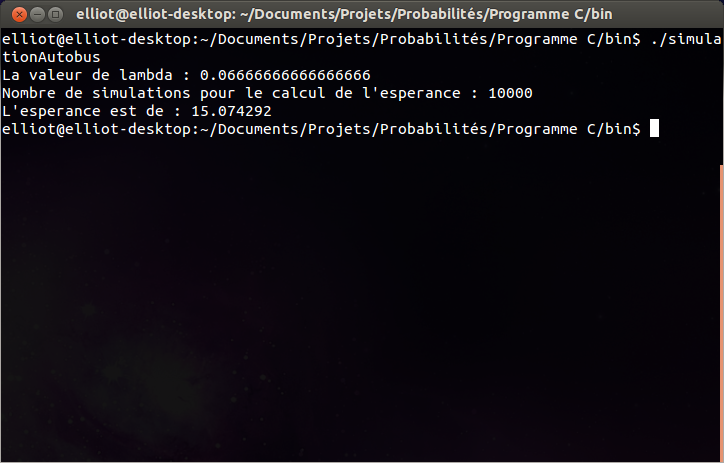
\includegraphics[scale = 0.38]{screen1.png}
  						\caption{Un premier calcul de $\mathbb{E}[A_{t}]$}
				\end{figure}

				C'est une valeur très étrange et très éloignée de celle estimée... Nous allons donc essayer de réitérer le calcul...
				\newpage


		\section{Approximation et conjecture de $\mathbb{E}[A_{t}]$}
			Au vu de la première valeur renvoyée par le programme, on peut penser que le hasard nous a joué un tour, on recommence donc l'opération mais cette fois-ci sur un million de simulations :
			\begin{figure}[!ht]
				\centering
  					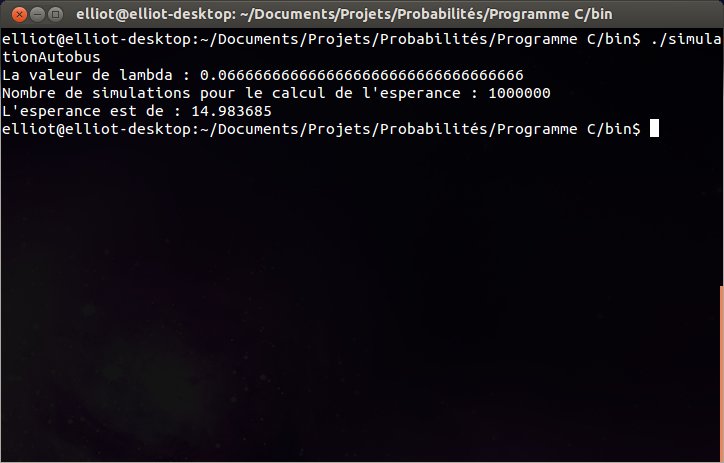
\includegraphics[scale = 0.38]{screen2.png}
  					\caption{Un deuxième calcul de $\mathbb{E}[A_{t}]$}
			\end{figure}

			Bigre ! Il semble que $\mathbb{E}[A_{t}] \approx 15$, c'est très surprenant car il s'agit de la moyenne de l'écart temporel entre deux bus.

			\begin{figure}[!ht]
					\centering
  						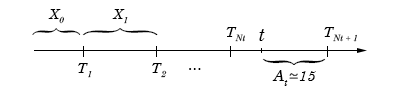
\includegraphics[scale = 0.45]{g5.png}
  						\caption{Représentation de $\mathbb{E}[A_{t}]$}
			\end{figure}
			Cela semble incroyable, on aurait donc :
			\[
				\mathbb{E}[A_{t}] = \frac{1}{\lambda}
			\]

			C'est très paradoxal dans le sens où un usager arrivant à un horaire $t$ attendra aussi longtemps (voir plus longtemps) son bus que s'il venait d'en rater un...
			La compagnie gérant les autobus peut donc se féliciter d'avoir un écart moyen de $15$ minutes entre chaque passage d'autobus, mais cela ne joue pas forcément en la faveur de leur clientèle !
			On peut assumer que ce résultat surprenant est dû à la distribution exponentielle des bus.
			Notre conjecture aurait-elle pu être la bonne si l'on avait supposé que l'écart moyen entre deux bus suivait une loi uniforme ?
			En changeant la simulation de $A_{t}$ par une loi uniforme sur un intervalle $[0;30]$, il en vient que :
			\begin{figure}[!ht]
				\centering
  					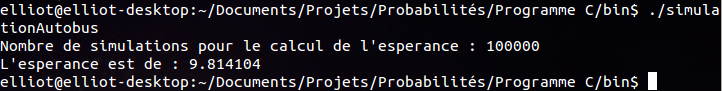
\includegraphics[scale = 0.38]{screen3.png}
  					\caption{Un calcul de $\mathbb{E}[A_{t}]$ avec des accroissements différents}
			\end{figure}

			Non plus ! 
			Décidément, le temps d'attente est toujours plus grand que l'espérance des $X_{n}$.
			On peut donc imaginer que cela vient du fait que lorsque l'on simule un horaire, il a beaucoup plus de chance de tomber dans un grand intervalle de temps que dans un petit.


	\chapter{Calcul de l'espérance de $A_{t}$}
		Dans cette partie, nous commencerons par calculer la loi de $A_{t}$ pour pouvoir ensuite étudier son espérance.
		On essayera enfin de lever complètement le paradoxe concernant l'espérance du temps d'attente en expliquant la raison pour laquelle l'intuition feint un résultat erroné.
	
		\section{Détermination de la loi de $A_{t}$}
			On sait que $A_{t}$ est le temps d'attente avant le prochain bus.
			Autrement dit, si l'on a raté le $n$ième bus, cela correspond au temps à attendre avant d'attraper le $(n+1)$ième bus :
			\[\begin{aligned}
				\forall \omega \in \Omega,\  \forall x \in \mathbb{R}_{+}, \ \omega \in \{A_{t} \leq x\} & \Leftrightarrow \exists n \in \mathbb{N}\ / \ \omega \in \{T_{n+1} > t \geq T_{n}\} \ et \ T_{n+1}(\omega) - t \leq x\\
																										 & \Leftrightarrow \exists n \in \mathbb{N}\ / \ \omega \in \{N_{t} = n\} \cap \{T_{n+1} - t \leq x\}\\
																										 & \Leftrightarrow \omega \in \bigcup_{n \geq 0} \{N_{t} = n\} \cap \{T_{n+1} - t \leq x\}\\
																										 & \Leftrightarrow \omega \in \{T_{N_{t}+1} - t \leq x\}
			\end{aligned}\]
			Ainsi :
			\[\boxed{
				A_{t} = T_{N_{t}+1} - t
			}\]
			\[\begin{array}{ccccc}
				A_{t} & : & \Omega & \to & \mathbb{R}_{+} \\
					  &   & \omega & \mapsto & T_{N_{t}+1}(\omega) - t\\
			\end{array}\]

			\begin{figure}[!ht]
				\centering
  					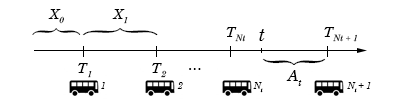
\includegraphics[scale=0.6]{g3.png}
  					\caption{Un schéma représentant $A_{t}$}
			\end{figure}

			On cherche la $f.d.r$ de $A_{t}$, c'est-à-dire : $\forall x \in \mathbb{R}, \ F_{A_{t}}(x) = \mathbb{P}(A_{t} \leq x) = 1 - \mathbb{P}(A_{t} > x)$.
			Nous allons ici plutôt nous intéresser à la fonction de survie de $A_{t}$, c'est-à-dire à $\mathbb{P}(A_{t} > x)$.
			On commence par remarquer que les $\{N_{t} = n\}$ forment une partition de $\Omega$, en effet :
			\begin{enumerate}
				\item $\forall (n, m) \in \mathbb{N}^{2}, \ (n \neq m \Rightarrow \{N_{t} = n\} \cap \{N_{t} = m\} = \varnothing)$
				\item $\Omega = \bigcup_{n \geq 0} \{N_{t} = n\}$
			\end{enumerate}
			Ainsi,
			\[
				\forall x \in \mathbb{R}_{+}, \ \mathbb{P}(A_{t} > x) = \mathbb{P}\left(\bigcup_{n \geq 0} \{A_{t} > x\} \cap \{N_{t} = n\}\right)
			\]
			Soit $n \in \mathbb{N}$ fixé. Calculons d'abord la probabilité de l'événement $\{A_{t} > x\} \cap \{N_{t} = n\}$ :
			\[\begin{aligned}
				\mathbb{P}(\{T_{N_{t}+1} - t > x\} \cap \{N_{t} = n\}) & = \mathbb{P}(\{T_{n+1} > t + x\} \cap \{N_{t} = n\})\\
																	   & = \mathbb{P}(\{T_{n+1} - T_{n} > t + x - T_{n}\} \cap \{N_{t} = n\}) \\
																	   & = \mathbb{P}(\{X_{n} > t + x - T_{n}\} \cap \{N_{t} = n\}) \\
			\end{aligned}\]
			Or,
			\[\begin{aligned}
				\omega \in \{X_{n} > t + x - T_{n}\} \cap \{N_{t} = n\} & \Leftrightarrow X_{n}(\omega) > t + x - T_{n}(\omega) \ et \ T_{n+1}(\omega) > t \geq T_{n}(\omega)\\
																		& \Leftrightarrow X_{n}(\omega) > x \ et \ N_{t}(\omega) = n 
			\end{aligned}\]
			Donc, comme les variables aléatoires $N_{t}$ et $X_{n}$ sont clairement indépendantes (le nombre de bus passés à l'instant $t$ ne dépend pas de l'écart temporel avec le prochain bus, ou encore la probabilité d'avoir un écart temporel supérieur à $x$ sachant que $n$ bus sont passés est la même que la probabilité d'avoir un écart temporel supérieur à $x$) :
			\[\begin{aligned}
				\mathbb{P}(\{T_{N_{t}+1} - t > x\} \cap \{N_{t} = n\}) & = \mathbb{P}(\{X_{n} > x\} \cap \{N_{t} = n\}) \\
																	   & = \mathbb{P}(X_{n} > x)\mathbb{P}(N_{t} = n) \\
																	   & = \left(1 - \left(1 - e^{-\lambda x}\right)\right)e^{-\lambda t}\frac{(\lambda t)^{n}}{n!} \\
																	   & = e^{-\lambda (t + x)}\frac{(\lambda t)^{n}}{n!} \\
			\end{aligned}\]
			Et donc, finalement :
			\[\begin{aligned}
				\mathbb{P}(A_{t} > x) & = \mathbb{P}\left(\bigcup_{n \geq 0} \{A_{t} > x\} \cap \{N_{t} = n\}\right)\\
									  & = \sum_{n \geq 0} \mathbb{P}(\{A_{t} > x\} \cap \{N_{t} = n\})\\
									  & = \sum_{n \geq 0} e^{-\lambda (t + x)}\frac{(\lambda t)^{n}}{n!}\\
									  & = e^{-\lambda (t + x)}\sum_{n \geq 0}\frac{(\lambda t)^{n}}{n!}\\
									  & = e^{-\lambda (t + x)}e^{\lambda t}\\
									  & = e^{-\lambda x}\\
			\end{aligned}\]
			D'où :
			\[\boxed{
				\forall x \in \mathbb{R}, \ F_{A_{t}}(x) = \mathbb{P}(A_{t} \leq x) = (1 - e^{-\lambda x})\mathbbm{1}_{\mathbb{R}_{+}}(x)
			}\]
			On remarque que $A_{t} \hookrightarrow \xi(\lambda)$ (car une loi est caractérisée par sa $f.d.r$).
			La loi de $A_{t}$ aurait pu être calculée un peu plus rapidement\footnote{Ce calcul est réalisé dans l'annexe C} en utilisant une variable aléatoire de comptage sur un intervalle quelconque.
		
		\section{Calcul de $\mathbb{E}[A_{t}]$}
			$A_{t} \hookrightarrow \xi(\lambda)$ ainsi, d'après le calcul effectué précédemment sur l'espérance d'une variable aléatoire exponentielle, on a : 
			\[\boxed{
				\mathbb{E}[A_{t}] = \frac{1}{\lambda}
			}\]
			Dans notre cas, cela nous donne : 
			\[\boxed{
				\mathbb{E}[A_{t}] = 15
			}\]
			Le temps d'attente moyen d'un usager à son arrêt est donc de $15$ minutes.

		\section{Comparaison avec les résultats précédents}
			On retrouve bien le résultat de notre deuxième conjecture, qui était en désaccord complet avec notre conjecture préliminaire.
			On avait émis comme hypothèse que cela était dû au fait que $t$ se retrouverait souvent dans un intervalle plus grand.
			Autrement dit, que la longueur moyenne de l'intervalle contenant $t$ serait plus grande que la longueur moyenne d'un intervalle.

			Pour vraiment lever le voile sur ce résultat paradoxal on se propose de calculer, justement, l'espérance de cet intervalle.
			Pour cela, on pose $B_{t}$ la variable aléatoire qui définit, lorsqu'un utilisateur arrive à une date $t > 0$ fixée, le temps déjà écoulé depuis le passage du bus qu'il a raté.
			Autrement dit,
			\[\begin{aligned}
				\forall \omega \in \Omega,\  \forall x \in \mathbb{R}_{+}, \ \omega \in \{B_{t} \leq x\} & \Leftrightarrow \exists n \in \mathbb{N}\ / \ \omega \in \{T_{n+1} >  t \geq T_{n}\} \ et \ t - T_{n}(\omega) \leq x\\
																										 & \Leftrightarrow \exists n \in \mathbb{N}\ / \ \omega \in \{N_{t} = n\} \cap \{t - T_{n} \leq x\}\\
																										 & \Leftrightarrow \omega \in \bigcup_{n \geq 0} \{N_{t} = n\} \cap \{t - T_{n} \leq x\}\\
																										 & \Leftrightarrow \omega \in \{t - T_{N_{t}} \leq x\}
			\end{aligned}\]
			Ainsi :
			\[\boxed{
				B_{t} = t - T_{N_{t}}
			}\]
			Et on remarque, justement, que :
			\[\boxed{
				A_{t} + B_{t} = X_{N_{t}}
			}\]
			La loi de $A_{t} + B_{t}$ est exactement la loi de l'intervalle contenant $t$.
			Par linéarité de l'espérance, il ne nous reste donc qu'à trouver la loi et l'espérance de $B_{t}$.
			On calcule, là encore, la fonction de survie de $B_{t}$, à $x \in \mathbb{R}_{+}$ fixé :
			\[\begin{aligned}
				\mathbb{P}(B_{t} > x) & = \mathbb{P}\left(\bigcup_{n \geq 0} \{B_{t} > x\} \cap \{N_{t} = n\}\right)\\
									  & = \sum_{n \geq 0} \mathbb{P}(\{B_{t} > x\} \cap \{N_{t} = n\})\\
									  & = \sum_{n \geq 0} \mathbb{P}(\{t - x > T_{n}\} \cap \{N_{t} = n\})\\
			\end{aligned}\]
			On distingue trois cas :
			\begin{itemize}
				\item Le cas où $x < t$.
				\item Le cas où $x > t$, ce qui implique que l'événement $\{B_{t} > x\}$ est équivalent à $\{0 > T_{N_{t}}\}$, ce qui est évidemment de probabilité nulle. Donc, pour $x > t$, $\mathbb{P}(\{B_{t} \leq x\}) = 1$.
				\item Le cas où $x = t$.
			\end{itemize}
			Pour $x < t$ :
			\[\begin{aligned}
				\mathbb{P}(B_{t} > x) & = \sum_{n \geq 0} \mathbb{P}(\{t - x > T_{n}\} \cap \{N_{t} = n\})\\
									  & = \sum_{n \geq 0} \mathbb{P}(\{t - x > T_{n}\} \cap \{T_{n} \leq t < T_{n+1}\})\\
									  & = \sum_{n \geq 0} \mathbb{P}(\{x - t + T_{n+1} < T_{n+1} - T_{n}\} \cap \{N_{t} = n\})\\
									  & = \sum_{n \geq 0} \mathbb{P}(\{x < X_{n}\} \cap \{N_{t} = n\})\\
									  & = \sum_{n \geq 0} \mathbb{P}(\{x < X_{n}\}) \mathbb{P}(\{N_{t} = n\})\\
									  & = \sum_{n \geq 0} e^{-\lambda x}e^{-\lambda t}\frac{(\lambda t)^{n}}{n!}\\
									  & = e^{-\lambda x}
			\end{aligned}\]
			Calculons $\mathbb{P}(B_{t} \leq t)$ :
			\[\begin{aligned}
				\mathbb{P}(B_{t} \leq t) & = \mathbb{P}(\{T_{N_{t}} \leq 0\})\\
										 & = \mathbb{P}(\{T_{N_{t}} = 0\})\\
									     & = \mathbb{P}(\{N_{t} = 0\})\\
									     & = e^{-\lambda t}
			\end{aligned}\]

			D'où:
			\[\boxed{
				\forall x \in \mathbb{R}, \ \mathbb{P}(B_{t} \leq x) = (1 - e^{-\lambda x})\mathbbm{1}_{0 \leq x < t}(x) + \mathbbm{1}_{x > t}(x) + e^{-\lambda t}\mathbbm{1}_{x = t}(x)
			}\]
			C'est une loi exponentielle tronquée en $t$.

			On en déduit la densité de $B_{t}$ :
			\[\begin{aligned}
				\forall x \in \mathbb{R}\setminus \{t\}, f_{B_{t}}(x) & = F_{B_{t}}'(x)\\
													                  & = \lambda e^{-\lambda x}\mathbbm{1}_{0 \leq x < t}(x)
			\end{aligned}\]
			Au point $x = t$, la fonction de répartition n'est pas continue et donc la densité n'existe pas.
			On dit que $B_{t}$ admet un atome de probabilité en $t$ : $\mathbb{P}(B_{t} \leq t) = \mathbb{P}(B_{t} = t) \neq 0$.

			Calculons $\mathbb{E}[B_{t}]$, par le théorème du transfert :
			\[\begin{aligned}
				\mathbb{E}[B_{t}] & = \int_{-\infty}^{\infty} xf_{B_{t}}(x)dx\\
								  & = \int_{0}^{t} \lambda x e^{-\lambda x}dx + tP(B_{t} = t)\\
								  & = \lambda \left(\left[ -\frac{x}{\lambda} e^{-\lambda x}\right]_{0}^{t} - 
   										\int_{0}^{t} -\frac{1}{\lambda} e^{-\lambda x} dx\right) + te^{-\lambda t}\\
                                  & = \lambda \left(-\frac{t}{\lambda}e^{-\lambda t} + \left[-\frac{1}{\lambda^{2}} e^{-\lambda x}\right]_{0}^{t}\right) + te^{\lambda t} \\
                                  & = \frac{1}{\lambda}(1 - e^{-\lambda t}) \\
			\end{aligned}\]

			Finalement,
			\[\boxed{
				\mathbb{E}[B_{t}] = \frac{1}{\lambda}(1 - e^{-\lambda t})
			}\]
			D'où :
			\[\boxed{
				\mathbb{E}[X_{N_{t}}] = \mathbb{E}[A_{t}] + \mathbb{E}[B_{t}] = \frac{1}{\lambda}(2 - e^{-\lambda t})
			}\]


			Ainsi, on voit que l'intervalle contenant $t$ est plus grand en moyenne qu'un intervalle quelconque !
			Et même, quand $t \rightarrow \infty$, il devient de longueur moyenne double !
			\begin{figure}[!ht]
				\centering
  					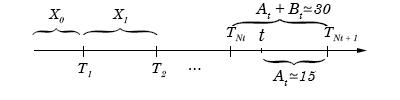
\includegraphics[scale=0.6]{g6.png}
  					\caption{L'espérance de la longueur de l'intervalle contenant $t$}
			\end{figure}

			Donc un usager arrive très souvent \og au mauvais moment \fg, surtout s'il arrive tard.
			Cela nous fait un peu penser à la loi de Murphy : \og Tout ce qui peut mal tourner, tournera mal \fg.

	
	\chapter*{Conclusion}
	\addcontentsline{toc}{chapter}{Conclusion} % ajouter la conclusion au sommaire
		Ce projet, d'une durée relativement limitée, nous aura néanmoins enseigné de nombreuses choses :
		\begin{itemize}
			\item Une maîtrise plus poussée des probabilités, une meilleure compréhension du cours.
			\item De nouvelles connaissances et une introduction au processus de Poisson que l'on verra en GM4.
			\item Une opportunité pour nous perfectionner en langage C.
			\item La compréhension d'un paradoxe surprenant.
			\item Une vision plus globale de la matière Probabilités-Statistiques (GM3) que nous continuerons d'étudier toute l'année.
		\end{itemize}

		Le calcul probabiliste est une branche qui nous tient à coeur dans le sens où l'on peut souvent appliquer la théorie mathématique à des situations bien concrètes.
		Les outils de calcul des probabilités mis à notre disposition nous ont permis ici de complètement lever le voile sur une situation très paradoxale.

		On a pu notamment mettre en évidence que le temps d'attente d'un passager à son arrêt de bus dépassait souvent les limites de sa patience, expliquant ainsi les vagues de colère fréquentes des usagers des réseaux de transports en commun.


	\appendix
	\addtocontents{toc}{\protect\setcounter{tocdepth}{0}} % profondeur table des matières annexes

	\chapter{La variable aléatoire de comptage dans un intervalle $N_{]a;b]}$}
		Nous allons ici généraliser le résultat trouvé pour $N_{t} = N_{[0;t]}$ dans la première partie de ce projet :
		\[
			\forall n \in \mathbb{N}, \ \mathbb{P}(N_{t} = n) = e^{-\lambda t}\frac{(\lambda t)^{n}}{n!}
		\]
		On admet ici que le processus de Poisson est stationnaire, c'est-à-dire que $\forall (s < t) \in \mathbb{R}_{+}^{2}$ :
		\[
			N_{t+s} - N_{s} \hookrightarrow N_{t}
		\]
		On remarque ensuite que : 
		\[\begin{aligned}
			N_{b} = N_{a} + N_{]a;b]} & \Leftrightarrow N_{]a;b]} = N_{[0;b]} - N_{[0;a]}\\
									  & \Leftrightarrow N_{]a;b]} = N_{[0;a + (b -a)]} - N_{[0;a]}\\
		\end{aligned}\]
		Comme $(b-a) \in \mathbb{R}^{+}$, on a :
		\[\boxed{
			N_{]a;b]} \hookrightarrow N_{(b-a)}
		}\]
		Et donc :
		\[\boxed{
			\forall n \in \mathbb{N}, \ \mathbb{P}(N_{]a;b] } = n) = e^{-\lambda (b-a)}\frac{(\lambda (b-a))^{n}}{n!}
		}\]

	\chapter{Une autre manière de calculer $I_{n}$}
		On rappelle que l'on voulait calculer, pour tout $n \in \mathbb{N}^{*}$ et $x \in \mathbb{R}_{+}$ fixé,
		\[
			I_{n}(x) = \int_{0}^{x} t^{n-1} e^{-\lambda t}dt
		\]
		Une façon astucieuse de résoudre ce problème est de poser, pour un polynôme $P$ de degré $n$ fixé :
		\[
			\forall x \in \mathbb{R}, \ D(x) = -\left[\sum_{k = 0}^{n} P^{(k)}(x)\right]e^{-x}
		\]
		Et alors, on peut remarquer que :
		\[\begin{aligned}
			D'(x) & = -\left[\sum_{k = 0}^{n-1} P^{(k+1)}(x)-\sum_{k = 0}^{n} P^{(k)}(x)\right]e^{-x} \\
				  & = -\left[\sum_{k = 1}^{n} P^{(k)}(x)-\sum_{k = 0}^{n} P^{(k)}(x)\right]e^{-x}\\
				  & = P(x)e^{-x}
		\end{aligned}\]
		On peut déduire de l'égalité précédente que :
		\[\begin{aligned}
			\int_{0}^{x} P(t)e^{-t}dt & = \int_{0}^{x} D'(t)dt\\
								 	  & = D(x) - D(0)\\
								 	  & = -\left[\sum_{k = 0}^{n} P^{(k)}(x)\right]e^{-x} + \sum_{k = 0}^{n} P^{(k)}(0)
		\end{aligned}\]
		On se donne le polynôme $P$ tel que $\forall t \in \mathbb{R}, \ P(t) = t^{n-1}$ de degré $n - 1$.
		Alors, en appliquant la formule ci-dessus :
		\[\begin{aligned}
			\int_{0}^{x} t^{n-1}e^{-t}dt & = -\left[x^{n-1} + (n-1)x^{n-2} + ... + (n-1)...2 x^{1} + (n-1)...1\right]e^{-x} + 0 + (n-1)...1\\
										 & = -\left[\sum_{k = 0}^{n-1} \frac{(n-1)!}{(n-1-k)!} x^{n-1-k}\right]e^{-x} + (n-1)!\\
										 & = -\left[\sum_{k = 0}^{n-1} \frac{(n-1)!}{k!} x^{k}\right]e^{-x} + (n-1)!\\
		\end{aligned}\]
		Par un changement de variable $u = \lambda t$ dans $I_{n}$, on a :
		\[\begin{aligned}
			I_{n}(x) & = \int_{0}^{x} t^{n-1} e^{-\lambda t}dt\\
					 & = \int_{0}^{\lambda x} (\frac{u}{\lambda})^{n-1} e^{-u}\frac{1}{\lambda}du\\
					 & = \frac{1}{\lambda^{n}}\int_{0}^{\lambda x} u^{n-1} e^{-u}du\\
					 & = \frac{1}{\lambda^{n}} \left(-\left[\sum_{k = 0}^{n-1} \frac{(n-1)!}{k!} (\lambda x)^{k}\right]e^{-\lambda x} + (n-1)!\right)\\
					 & = -\left[\sum_{k = 0}^{n-1} \frac{(n-1)!}{k!} \frac{(\lambda x)^{k}}{\lambda^{n}}\right]e^{-\lambda x} + \frac{(n-1)!}{\lambda^{n}}
		\end{aligned}\]
		Ainsi on retrouve bien le résultat que l'on avait démontré par récurrence :
		\[\boxed{
			\forall n \in \mathbb{N}^{*}, \ \forall x \in \mathbb{R}, \ I_{n}(x) = \left(\frac{(n-1)!}{\lambda^{n}} -\left[\sum_{k = 0}^{n-1} \frac{(n-1)!}{k!} \frac{(\lambda x)^{k}}{\lambda^{n}}\right]e^{-\lambda x}\right)\mathbbm{1}_{\mathbb{R}_{+}}(x)
		}\]

	\chapter{Une autre façon de déterminer la loi de $A_{t}$ et de $B_{t}$}
		On cherche ici la fonction de répartition de $A_{t}$ et de $B_{t}$.
		La démonstration est presque la même, sauf qu'ici on utilise la variable aléatoire de comptage sur un intervalle, ce qui nous donne la solution un tout petit peu plus rapidement.
		Encore une fois, on se ramène à la fonction de survie $\mathbb{P}(A_{t} > x)$.
		Soit $x \in \mathbb{R}^{+}$ :
		\[\begin{aligned}
			\mathbb{P}(A_{t} > x) & = \mathbb{P}\left(\bigcup_{n \geq 0} \{A_{t} > x\} \cap \{N_{t} = n\}\right)\\
								  & = \sum_{n \geq 0} \mathbb{P}(\{T_{n+1} > t + x \geq t \geq T_{n}\})\\
								  & = \sum_{n \geq 0} \mathbb{P}(\{N_{]t;t+x]} = 0\} \cap \{N_{t} = n\})\\
								  & = \sum_{n \geq 0} \mathbb{P}(\{N_{]t;t+x]} = 0\}) \mathbb{P}(\{N_{t} = n\})\\
		\end{aligned}\]
		Il y a indépendance entre $N_{]t;t+x]}$ et $N_{t}$ car le nombre de passages d'autobus entre $t$ et $(t+x)$ ne dépend pas du nombre de bus passés jusqu'à la date $t$.
		\[\begin{aligned}
			\mathbb{P}(A_{t} > x) & = \sum_{n \geq 0} \mathbb{P}(\{N_{]t;t+x]} = 0\}) \mathbb{P}(\{N_{t} = n\})\\
							      & = \sum_{n \geq 0} e^{-\lambda (t+x - t)} e^{-\lambda t} \frac{(\lambda t)^{n}}{n!}\\
							      & = e^{-\lambda x}\\
		\end{aligned}\]
		D'où, pour tout $x \in \mathbb{R}$ :
		\[\boxed{
			\mathbb{P}(A_{t} \leq x) = (1 - e^{-\lambda x})\mathbbm{1}_{\mathbb{R}_{+}}(x)
		}\]
		On retrouve bien la loi de $A_{t}$ trouvée en troisième partie de ce projet.

		Pour ce qui est de $B_{t}$, on distingue encore les trois cas : $x < t$, $x > t$ et $x = t$.\\
		Soit $x < t$ :
		\[\begin{aligned}
			\mathbb{P}(B_{t} > x) & = \mathbb{P}\left(\bigcup_{n \geq 0} \{B_{t} > x\} \cap \{N_{t} = n\}\right)\\
								  & = \sum_{n \geq 0} \mathbb{P}(\{t - x > T_{n}\} \cap \{T_{n+1} > t \geq T_{n}\})\\
								  & = \sum_{n \geq 0} \mathbb{P}(\{T_{n+1} > t > t - x \geq T_{n}\})\\
								  & = \sum_{n \geq 0} \mathbb{P}(\{N_{]t-x;t]} = 0\}) \mathbb{P}(\{N_{t-x} = n\})\\
								  & = \sum_{n \geq 0} e^{-\lambda (t - (t-x))} e^{-\lambda (t - x)} \frac{(\lambda (t - x))^{n}}{n!}\\
								  & = e^{-\lambda x}
		\end{aligned}\]
		Pour $x > t$ et $x = t$, on a toujours respectivement $\mathbb{P}(\{B_{t} \leq x\}) = 1$ et $\mathbb{P}(\{B_{t} \leq t\}) = e^{-\lambda t}$.
		D'où, pour tout $x \in \mathbb{R}$ :
		\[\boxed{
			\mathbb{P}(B_{t} \leq x) = (1 - e^{-\lambda x})\mathbbm{1}_{0 \leq x < t}(x) + \mathbbm{1}_{x > t}(x) + e^{-\lambda t}\mathbbm{1}_{x = t}(x)
		}\]
		On retrouve bien la loi exponentielle tronquée en $t$ précédemment calculée.

	
	\chapter{Programme de simulation}
		\lstset{language=C,
			inputencoding=utf8/latin1
			}

		\section{Les headers}
			\subsection{IHM}
				Fichier : IHM.h
	
				\lstinputlisting{src/IHM.h}
			
			\subsection{Simulation}
				Fichier : simulation.h
	
				\lstinputlisting{src/simulation.h}
	
		\section{Programme principal}
			Fichier : main.c
	
			\lstinputlisting{src/main.c}

		\section{Le module IHM}
			Fichier : IHM.c
	
			\lstinputlisting{src/IHM.c}

		\section{Le module simulation}
			Fichier : simulation.c
	
			\lstinputlisting{src/simulation.c}
	
		\section{Le makefile}
			Fichier : Makefile
			\lstset{language=make} 
		
			\lstinputlisting{src/Makefile}
	
	\begin{thebibliography}{9}
	\addcontentsline{toc}{chapter}{Bibliographie} % ajouter la bibliographie au sommaire
	
		\bibitem{Cours 01}
			\emph{Mohamed El Machkouri},
			\textit{Cours de Probabilités/Statistiques},
			Institut National des Sciences Appliquées de Rouen.
	
		\bibitem{Article 01}
			\emph{E. Lecarbier, S. Robin},
			\textit{Un bref aperçu du processus de Poisson},
			AgroParisTech, 2007.

		\bibitem{Article 02}
			\emph{F. Testard},
			\textit{Modèles exponentiels},
			Université de La Rochelle, 2010.

		\bibitem{Lien Internet 01}
			\url{http://www.universalis.fr/encyclopedie/simeon-denis-poisson/}
			(Valide à la date du 20/11/2013)
			Biographie de Siméon Denis Poisson.

		\bibitem{Lien Internet 02}
			\url{http://nestor.coventry.ac.uk/~nhunt/poisson/history.html}
			(Valide à la date du 20/11/2013)
			Une bref histoire concernant la distribution de Poisson.

		\bibitem{Lien Internet 03}
			\url{http://images.math.cnrs.fr/Poisson.html}
			(Valide à la date du 20/11/2013)
			Quelques détails sur l'ouvrage de Poisson \og Recherches sur la probabilité des jugements en matière criminelle et matière civile \fg.

		\bibitem{Lien Internet 04}
			\url{http://www.math.nyu.edu/faculty/varadhan/spring06/spring06.1.pdf}
			(Valide à la date du 20/11/2013)
			Un pdf bien détaillé sur le processus de Poisson.

		\bibitem{Lien Internet 05}
			\url{http://www.math.uah.edu/stat/poisson/}
			(Valide à la date du 20/11/2013)
			Un cours sur le processus de Poisson.

		\bibitem{Lien Internet 06}
			\url{http://www.netlab.tkk.fi/opetus/s383143/kalvot/E_poisson.pdf}
			(Valide à la date du 20/11/2013)
			Un pdf avec des explications du processus de Poisson et ses propriétés.
	
	
	\end{thebibliography}


\end{document} % fin du document
